% Edit these commands before the final exam delivery.
\documentclass[11pt,aspectratio=169,t]{beamer}

\usepackage[T1]{fontenc}
\usepackage{lmodern}
\usepackage{microtype}
\usepackage{graphicx}
\usepackage{booktabs}
\usepackage{array}
\usepackage{amsmath}
\usepackage{tikz}
\usepackage{pgfplots}
\usepackage{pgfplotstable}
\usepackage{xcolor}
\usetikzlibrary{arrows.meta,positioning,calc,fit,backgrounds,matrix}
\pgfplotsset{compat=1.18}

\newcommand{\StudentName}{Student Name}
\newcommand{\DegreeProgramme}{Degree Programme}
\newcommand{\AcademicYear}{Academic Year 2025--2026}
\newcommand{\SupervisorName}{Supervisor Name}

\definecolor{Navy}{HTML}{102A43}
\definecolor{Blue}{HTML}{2878B5}
\definecolor{BlueLight}{HTML}{DCEEFF}
\definecolor{Orange}{HTML}{F28E2B}
\definecolor{OrangeLight}{HTML}{FCE8D2}
\definecolor{Green}{HTML}{2E8B57}
\definecolor{GreenLight}{HTML}{DDF2E6}
\definecolor{Purple}{HTML}{7A5195}
\definecolor{PurpleLight}{HTML}{EEE5F4}
\definecolor{Ink}{HTML}{243B53}
\definecolor{Muted}{HTML}{627D98}
\definecolor{Rule}{HTML}{D9E2EC}
\definecolor{Canvas}{HTML}{F8FAFC}
\definecolor{UnisiRed}{HTML}{B00020}

\setbeamercolor{normal text}{fg=Ink,bg=white}
\setbeamercolor{frametitle}{fg=Navy,bg=white}
\setbeamercolor{title}{fg=Navy}
\setbeamercolor{subtitle}{fg=Muted}
\setbeamercolor{structure}{fg=Blue}
\setbeamercolor{alerted text}{fg=Orange}
\setbeamerfont{title}{series=\bfseries,size=\LARGE}
\setbeamerfont{subtitle}{size=\large}
\setbeamerfont{frametitle}{series=\bfseries,size=\Large}
\setbeamertemplate{navigation symbols}{}
\setbeamertemplate{itemize item}{\color{Blue}\small\raise0.2ex\hbox{\textbullet}}
\setbeamertemplate{itemize subitem}{\color{Muted}\scriptsize\raise0.2ex\hbox{\textbullet}}
\setlength{\leftmargini}{1.2em}
\setlength{\leftmarginii}{1.1em}

\setbeamertemplate{frametitle}{%
  \vspace{0.25cm}\insertframetitle\par
  \vspace{0.10cm}{\color{Rule}\rule{\textwidth}{0.6pt}}
}
\setbeamertemplate{footline}{%
  \leavevmode
  \hbox{%
    \begin{beamercolorbox}[wd=.82\paperwidth,ht=2.7ex,dp=1.2ex,leftskip=.55cm]{author in head/foot}%
      \color{Muted}\scriptsize Real vs. Synthetic Classification from Stable Diffusion Features
    \end{beamercolorbox}%
    \begin{beamercolorbox}[wd=.18\paperwidth,ht=2.7ex,dp=1.2ex,rightskip=.55cm plus1fil]{date in head/foot}%
      \color{Muted}\scriptsize\insertframenumber/\inserttotalframenumber
    \end{beamercolorbox}%
  }
}

\tikzset{
  proc/.style={draw=Rule, very thick, rounded corners=2pt, fill=Canvas,
    align=center, inner xsep=5pt, inner ysep=4pt, font=\scriptsize, minimum height=0.72cm},
  procblue/.style={proc, draw=Blue, fill=BlueLight},
  procgreen/.style={proc, draw=Green, fill=GreenLight},
  procpurple/.style={proc, draw=Purple, fill=PurpleLight},
  procorange/.style={proc, draw=Orange, fill=OrangeLight},
  flow/.style={-{Latex[length=2.2mm]}, line width=0.8pt, draw=Muted},
  dashflow/.style={flow, dashed},
  note/.style={font=\scriptsize, text=Muted, align=center}
}

\newcommand{\keymetric}[3]{%
  \begin{minipage}[t]{0.44\linewidth}\centering
    {\color{#1}\bfseries\fontsize{22}{24}\selectfont #2}\par
    \vspace{0.8mm}{\color{Muted}\scriptsize #3}
  \end{minipage}%
}

\newcommand{\confmatrix}[5]{%
\begin{tikzpicture}[font=\scriptsize]
  \node[font=\bfseries,text=Navy] at (1.35,2.95) {#1};
  \fill[Blue!82] (0,1.25) rectangle (1.25,2.5);
  \fill[Blue!8]  (1.25,1.25) rectangle (2.5,2.5);
  \fill[Blue!8]  (0,0) rectangle (1.25,1.25);
  \fill[Blue!92] (1.25,0) rectangle (2.5,1.25);
  \draw[Rule,thick] (0,0) grid[step=1.25] (2.5,2.5);
  \node[text=white,font=\bfseries] at (.625,1.875) {#2};
  \node[font=\bfseries] at (1.875,1.875) {#3};
  \node[font=\bfseries] at (.625,.625) {#4};
  \node[text=white,font=\bfseries] at (1.875,.625) {#5};
  \node[font=\tiny] at (.625,-.20) {real};
  \node[font=\tiny] at (1.875,-.20) {fake};
  \node[font=\tiny,rotate=90] at (-.22,1.875) {real};
  \node[font=\tiny,rotate=90] at (-.22,.625) {fake};
  \node[font=\tiny,text=Muted] at (1.25,-.48) {Predicted};
  \node[font=\tiny,text=Muted,rotate=90] at (-.50,1.25) {True};
\end{tikzpicture}%
}

\title{Real vs. Synthetic Image Classification\\from Stable Diffusion Feature Maps}
\subtitle{A comparison of tabular, spatial, and ensemble learning approaches}
\author{\StudentName}
\institute{University of Siena\\Advanced Machine Learning}
\date{\AcademicYear}

\begin{document}

% 1
\begin{frame}[plain]
  \begin{tikzpicture}[remember picture,overlay]
    \fill[white] (current page.south west) rectangle (current page.north east);
    \fill[UnisiRed] (current page.south west) rectangle ([xshift=0.22cm]current page.north west);
    \fill[Navy] ([yshift=0.34cm]current page.south west) rectangle ([yshift=0.41cm]current page.south east);
    \node[anchor=north west] at ([xshift=0.85cm,yshift=-0.52cm]current page.north west)
      {
\includegraphics[height=2.12cm,keepaspectratio]{../docs/LOGO_UNISI_VERTICALE_NERO_0.pdf}};
    \node[anchor=north west,text width=10.7cm,align=left,text=Navy,font=\bfseries\large]
      at ([xshift=4.35cm,yshift=-0.65cm]current page.north west)
      {Dipartimento di Ingegneria dell'Informazione\\[-1mm]e Scienze Matematiche};
    \draw[Rule,line width=0.6pt]
      ([xshift=4.35cm,yshift=-1.76cm]current page.north west) --
      ([xshift=-0.85cm,yshift=-1.76cm]current page.north east);
    \draw[Navy,line width=1.35pt]
      ([xshift=4.35cm,yshift=-1.88cm]current page.north west) --
      ([xshift=-0.85cm,yshift=-1.88cm]current page.north east);
    \node[anchor=north west,text=Ink,font=\small]
      at ([xshift=4.35cm,yshift=-2.04cm]current page.north west)
      {Degree programme: \textbf{\DegreeProgramme}};
    \node[anchor=north west,text=Ink,font=\small]
      at ([xshift=4.35cm,yshift=-2.55cm]current page.north west)
      {Course: \textbf{Advanced Machine Learning}};

    \node[anchor=north,text width=14.2cm,align=center,text=Navy,font=\bfseries\fontsize{20}{23}\selectfont]
      at ([yshift=-3.43cm]current page.north)
      {Real vs. Synthetic Image Classification\\[0.5mm]from Stable Diffusion Feature Maps};
    \node[anchor=north,text width=13cm,align=center,text=Muted,font=\scriptsize]
      at ([yshift=-5.05cm]current page.north)
      {A comparison of tabular, spatial, and ensemble learning approaches};

    \node[anchor=south west,text=Muted,font=\scriptsize]
      at ([xshift=0.95cm,yshift=1.38cm]current page.south west) {SUPERVISOR};
    \node[anchor=south west,text=Navy,font=\bfseries\normalsize]
      at ([xshift=0.95cm,yshift=0.96cm]current page.south west) {\SupervisorName};
    \node[anchor=south east,text=Muted,font=\scriptsize]
      at ([xshift=-0.95cm,yshift=1.38cm]current page.south east) {CANDIDATE};
    \node[anchor=south east,text=Navy,font=\bfseries\normalsize]
      at ([xshift=-0.95cm,yshift=0.96cm]current page.south east) {\StudentName};
    \node[anchor=south,text=Muted,font=\bfseries\small]
      at ([yshift=0.52cm]current page.south) {\AcademicYear};
  \end{tikzpicture}
\end{frame}

% 2
\begin{frame}{Research question}
  \begin{columns}[T,onlytextwidth]
    \column{0.45\textwidth}
      \vspace{0.25cm}
      \small
      \begin{itemize}
        \item Diffusion models encode rich internal representations.
        \item The reference study found the clearest real/fake separation in the first decoder layer at \(16\times16\) resolution.
        \item This project turns that observation into a supervised binary classification task.
      \end{itemize}
      \vspace{0.35cm}
      {\color{Navy}\bfseries\small Can a calibrated local ensemble match a higher-capacity ConvNeXt classifier?}
    \column{0.53\textwidth}
      \centering
      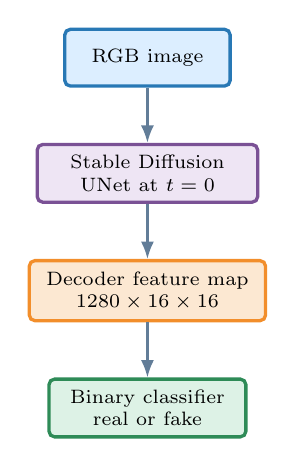
\begin{tikzpicture}[node distance=7mm]
        \node[procblue,minimum width=2.1cm] (im) {RGB image};
        \node[procpurple,below=of im,minimum width=2.8cm] (sd) {Stable Diffusion\\UNet at \(t=0\)};
        \node[procorange,below=of sd,minimum width=3.0cm] (fm) {Decoder feature map\\\(1280\times16\times16\)};
        \node[procgreen,below=of fm,minimum width=2.5cm] (cl) {Binary classifier\\real or fake};
        \draw[flow] (im)--(sd); \draw[flow] (sd)--(fm); \draw[flow] (fm)--(cl);
      \end{tikzpicture}
  \end{columns}
  \vfill
  {\tiny\color{Muted}Feature-layer motivation adapted from Bonechi, Andreini, and Toniella Corradini, ``Comparing Real and Synthetic Image Representations in Stable Diffusion Models.''}
\end{frame}

% 3
\begin{frame}{Dataset and input representation}
  \begin{columns}[T,onlytextwidth]
    \column{0.48\textwidth}
      \scriptsize
      \begin{tabular}{@{}p{1.25cm}p{3.55cm}r@{}}
        \toprule
        \textbf{Class} & \textbf{Sources} & \textbf{Samples}\\
        \midrule
        Real & Pascal VOC, COCO & 1,654\\
        Fake & DALL-E 3, Midjourney, SD 1.4/1.5 & 2,383\\
        \midrule
        Total & Six source datasets & 4,037\\
        \bottomrule
      \end{tabular}\par
      \vspace{0.28cm}
      \begin{itemize}
        \item One sample: \(1280\times16\times16\) float32 tensor.
        \item 327,680 values per sample (about 1.25 MiB); arrays total 4.93 GiB and use memory mapping.
        \item Positive class: \textbf{fake}; balanced accuracy addresses the moderate imbalance.
      \end{itemize}
    \column{0.49\textwidth}
      \centering
      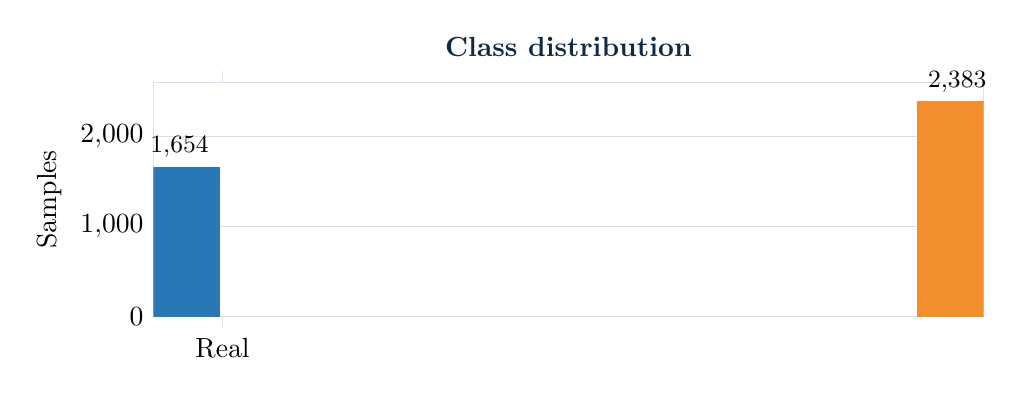
\begin{tikzpicture}
        \begin{axis}[
          width=\linewidth,height=4.55cm,
          ybar,bar width=29pt,ymin=0,ymax=2600,
          ylabel={Samples},symbolic x coords={Real,Fake},xtick=data,
          nodes near coords,nodes near coords align={vertical},
          axis line style={draw=Rule},tick style={draw=Rule},
          ymajorgrids=true,grid style={Rule},
          every node near coord/.append style={font=\small},
          title={Class distribution},title style={font=\bfseries,color=Navy}
        ]
          \addplot[fill=Blue,draw=Blue] coordinates {(Real,1654)};
          \addplot[fill=Orange,draw=Orange] coordinates {(Fake,2383)};
        \end{axis}
      \end{tikzpicture}
      {\scriptsize\color{Muted}Real: 41.0\% \quad Fake: 59.0\%}
  \end{columns}
\end{frame}

% 4
\begin{frame}{Shared evaluation protocol}
  \centering
  \vspace{0.25cm}
  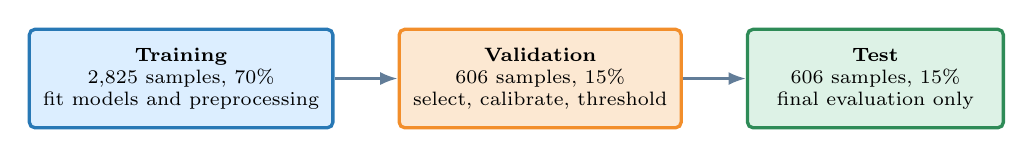
\begin{tikzpicture}[node distance=8mm]
    \node[procblue,minimum width=3.25cm,minimum height=1.25cm] (tr) {\textbf{Training}\\2,825 samples, 70\%\\fit models and preprocessing};
    \node[procorange,right=of tr,minimum width=3.25cm,minimum height=1.25cm] (va) {\textbf{Validation}\\606 samples, 15\%\\select, calibrate, threshold};
    \node[procgreen,right=of va,minimum width=3.25cm,minimum height=1.25cm] (te) {\textbf{Test}\\606 samples, 15\%\\final evaluation only};
    \draw[flow] (tr)--(va); \draw[flow] (va)--(te);
  \end{tikzpicture}
  \vspace{0.75cm}
  \begin{columns}[T,onlytextwidth]
    \column{0.49\textwidth}
      \begin{itemize}
        \item One stratified split, seed 42.
        \item Stable sample IDs and shared split hash.
        \item Training-only fitted preprocessing.
      \end{itemize}
    \column{0.49\textwidth}
      \begin{itemize}
        \item Validation balanced accuracy drives every model choice.
        \item No augmentation, oversampling, SMOTE, MixUp, or CutMix.
        \item Test remains isolated until decisions are frozen.
      \end{itemize}
  \end{columns}
  \vfill
  {\color{Navy}\bfseries The shared data contract makes comparisons leakage-aware and directly aligned.}
\end{frame}

% 5
\begin{frame}{The feature maps contain a strong class signal}
  \begin{columns}[T,onlytextwidth]
    \column{0.41\textwidth}
      \keymetric{Blue}{60.9\%}{channels with \(|d|\geq0.2\)}\hfill
      \keymetric{Orange}{20.3\%}{channels with \(|d|\geq0.5\)}
      \vspace{0.55cm}
      \begin{itemize}
        \item No NaNs, infinities, or exact duplicate samples.
        \item Four global statistics already yield \textbf{0.7332} validation balanced accuracy and \textbf{0.8019} ROC-AUC.
        \item Strong performance may include source or preprocessing confounders.
      \end{itemize}
    \column{0.56\textwidth}
      \centering
      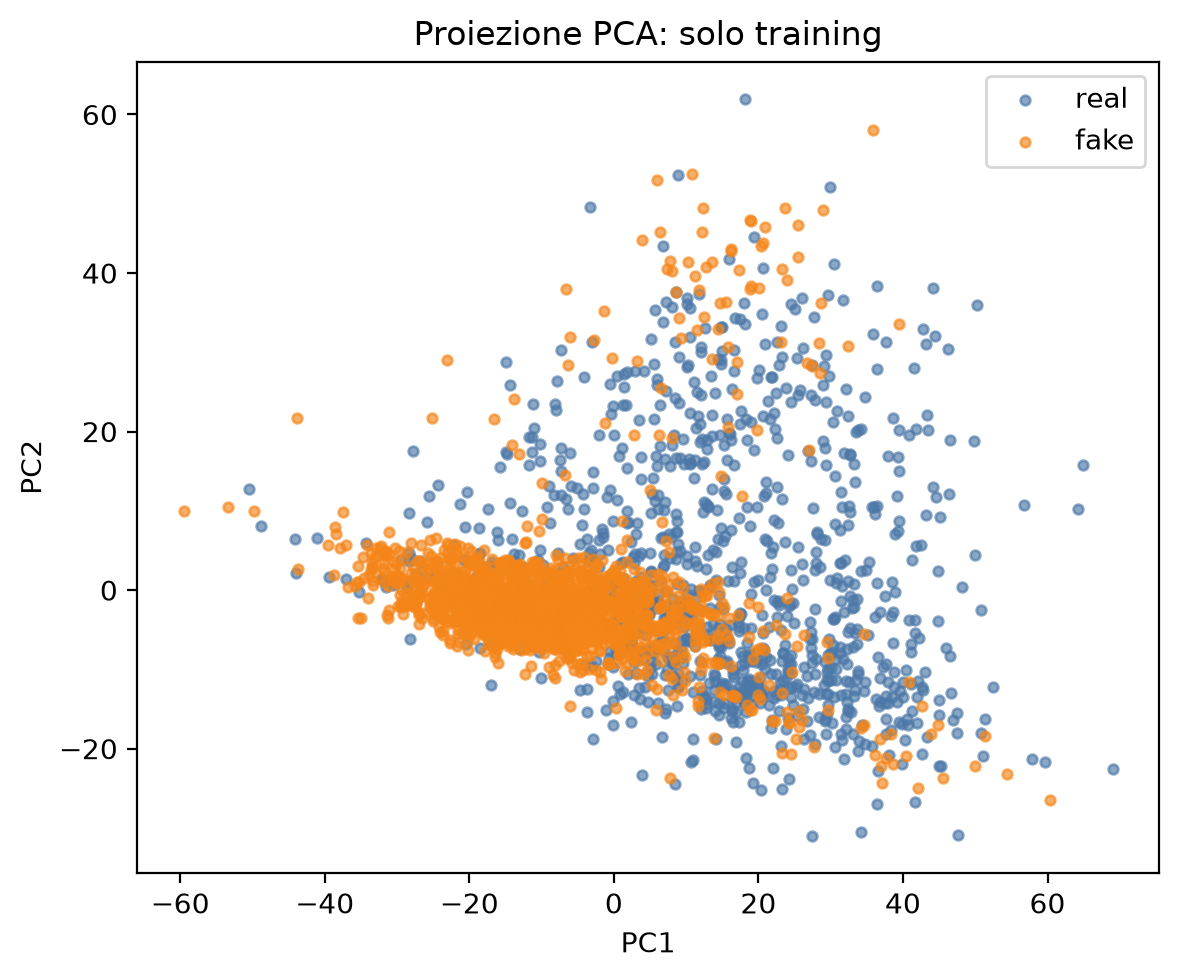
\includegraphics[height=4.65cm,keepaspectratio,trim=0 0 0 46,clip]{../results/dataset_exploration/seed42_20260916T132745Z/figures/pca_projection_train.png}
      \vspace{-0.15cm}
      {\scriptsize\color{Muted}Training-set PCA shows partial separation and substantial overlap.}
  \end{columns}
\end{frame}

% 6
\begin{frame}{GAP and mean+std descriptors}
  \centering
  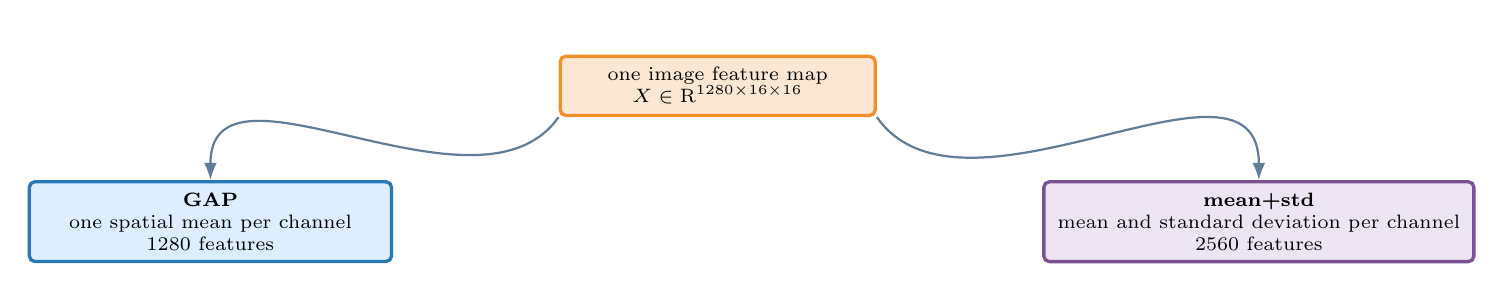
\begin{tikzpicture}[node distance=8mm]
    \node[procorange,minimum width=4.0cm] (x) {one image feature map\\\(X\in\mathrm{R}^{1280\times16\times16}\)};
    \node[procblue,below left=8mm and 21mm of x,minimum width=4.6cm] (gap) {\textbf{GAP}\\one spatial mean per channel\\\(1280\) features};
    \node[procpurple,below right=8mm and 21mm of x,minimum width=4.8cm] (ms) {\textbf{mean+std}\\mean and standard deviation per channel\\\(2560\) features};
    \draw[flow] (x.south west) to[out=-125,in=90] (gap.north);
    \draw[flow] (x.south east) to[out=-55,in=90] (ms.north);
  \end{tikzpicture}
  \vspace{0.08cm}
  \begin{columns}[T,onlytextwidth]
    \column{0.48\textwidth}
      {\color{Blue}\bfseries Global Average Pooling}
      \vspace{-0.08cm}
      {\small\[
        g_c=\frac{1}{HW}\sum_{h=1}^{H}\sum_{w=1}^{W}X_{c,h,w}
      \]}
      \scriptsize
      \textbf{What it captures.} The average activation of each channel.\par\smallskip
      \textbf{Why use it.} It produces a compact, position-independent summary and tests whether channel presence alone separates real and fake images.\par\smallskip
      \textbf{How it is used.} The SVM evaluated GAP and mean+std, then selected \textbf{GAP} on validation.
    \column{0.48\textwidth}
      {\color{Purple}\bfseries Channel mean and spread}
      \vspace{-0.08cm}
      {\scriptsize\[
        \mu_c=g_c,\qquad
        \sigma_c=\sqrt{\frac{1}{HW}\sum_{h,w}(X_{c,h,w}-\mu_c)^2}
      \]}
      \scriptsize
      \textbf{What it captures.} The channel mean plus its spatial variation, concatenated as \([\mu_1,\ldots,\mu_C,\sigma_1,\ldots,\sigma_C]\).\par\smallskip
      \textbf{Why use it.} It adds distribution spread without expanding to all 327,680 spatial values.\par\smallskip
      \textbf{How it is used.} XGBoost selected \textbf{mean+std} after comparing both summaries. The MLP also uses mean+std.
  \end{columns}
  \vfill
  {\scriptsize\color{Navy}\bfseries Each image becomes one feature vector. Both summaries discard the spatial arrangement, which the CNN and ConvNeXt retain.}
\end{frame}

% 7
\begin{frame}{Five models and three input representations}
  \centering
  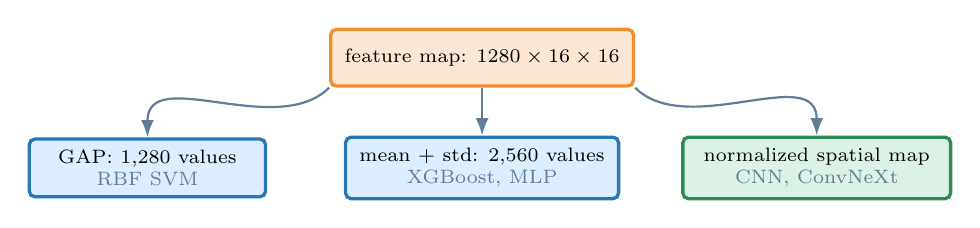
\begin{tikzpicture}
    \node[procorange,minimum width=3.0cm] (x) at (0,0.45) {feature map: \(1280\times16\times16\)};
    \node[procblue,minimum width=3.0cm] (gap) at (-4.25,-0.95) {GAP: 1,280 values\\\textcolor{Muted}{RBF SVM}};
    \node[procblue,minimum width=3.2cm] (ms) at (0,-0.95) {mean + std: 2,560 values\\\textcolor{Muted}{XGBoost, MLP}};
    \node[procgreen,minimum width=3.4cm] (sp) at (4.25,-0.95) {normalized spatial map\\\textcolor{Muted}{CNN, ConvNeXt}};
    \draw[flow] (x.south west) to[out=-135,in=90] (gap.north);
    \draw[flow] (x.south) -- (ms.north);
    \draw[flow] (x.south east) to[out=-45,in=90] (sp.north);
  \end{tikzpicture}
  \vspace{0.20cm}
  \scriptsize
  \begin{tabular}{@{}p{3.0cm}p{3.5cm}p{6.0cm}@{}}
        \toprule
        \textbf{Model} & \textbf{Input} & \textbf{Role}\\
        \midrule
        RBF SVM & GAP & kernel baseline, ensemble\\
        XGBoost & mean + std & tree baseline, ensemble\\
        MLP & mean + std & dense neural baseline\\
        CNN spatial head & full map & compact spatial, ensemble\\
        Compact ConvNeXt & full map & high-capacity reference\\
        \bottomrule
  \end{tabular}\par
  \vspace{0.28cm}
  {\small\color{Navy}\bfseries Global summaries test whether spatial detail is necessary. Spatial networks retain the full \(16\times16\) layout.}
\end{frame}

% 7
\begin{frame}{RBF SVM pipeline}
  \centering
  \resizebox{0.97\textwidth}{!}{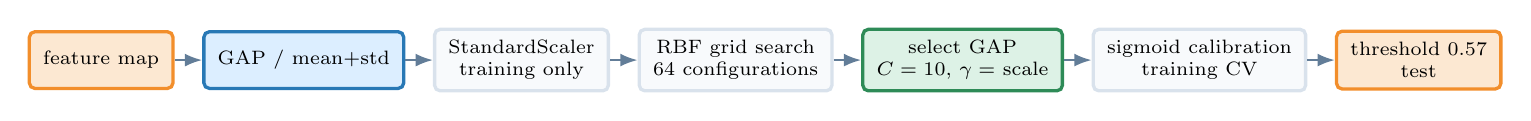
\begin{tikzpicture}[node distance=3.5mm]
    \node[procorange] (a) {feature map};
    \node[procblue,right=of a] (b) {GAP / mean+std};
    \node[proc,right=of b] (c) {StandardScaler\\training only};
    \node[proc,right=of c] (d) {RBF grid search\\64 configurations};
    \node[procgreen,right=of d] (e) {select GAP\\\(C=10\), \(\gamma=\) scale};
    \node[proc,right=of e] (f) {sigmoid calibration\\training CV};
    \node[procorange,right=of f] (g) {threshold 0.57\\test};
    \draw[flow] (a)--(b); \draw[flow] (b)--(c); \draw[flow] (c)--(d);
    \draw[flow] (d)--(e); \draw[flow] (e)--(f); \draw[flow] (f)--(g);
  \end{tikzpicture}}
  \vspace{0.75cm}
  \begin{columns}[T,onlytextwidth]
    \column{0.55\textwidth}
      \begin{itemize}
        \item Optional PCA was evaluated inside the pipeline and rejected by validation.
        \item The calibrated score estimates the probability of the fake class.
        \item The simplest representation produced the strongest individual model.
      \end{itemize}
    \column{0.42\textwidth}
      \centering
      \keymetric{Blue}{0.9722}{test balanced accuracy}
      \keymetric{Green}{0.9971}{test ROC-AUC}
      \vspace{0.45cm}
      {\scriptsize\color{Muted}Test errors: 2 false positives and 17 false negatives.}
  \end{columns}
\end{frame}

% 8
\begin{frame}{XGBoost pipeline}
  \centering
  \resizebox{0.97\textwidth}{!}{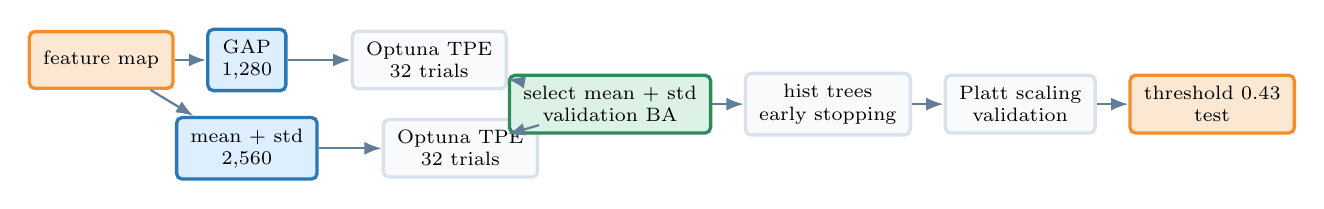
\begin{tikzpicture}[node distance=4mm]
    \node[procorange] (a) {feature map};
    \node[procblue,right=of a] (b1) {GAP\\1,280};
    \node[procblue,below=3mm of b1] (b2) {mean + std\\2,560};
    \node[proc,right=8mm of b1] (c1) {Optuna TPE\\32 trials};
    \node[proc,right=8mm of b2] (c2) {Optuna TPE\\32 trials};
    \node[procgreen,right=8mm of $(c1)!0.5!(c2)$] (d) {select mean + std\\validation BA};
    \node[proc,right=of d] (e) {hist trees\\early stopping};
    \node[proc,right=of e] (f) {Platt scaling\\validation};
    \node[procorange,right=of f] (g) {threshold 0.43\\test};
    \draw[flow] (a)--(b1); \draw[flow] (a)--(b2); \draw[flow] (b1)--(c1); \draw[flow] (b2)--(c2);
    \draw[flow] (c1)--(d); \draw[flow] (c2)--(d); \draw[flow] (d)--(e); \draw[flow] (e)--(f); \draw[flow] (f)--(g);
  \end{tikzpicture}}
  \vspace{0.35cm}
  \begin{columns}[T,onlytextwidth]
    \column{0.49\textwidth}
      \small
      \begin{tabular}{@{}lr@{}}
        \toprule
        max depth & 4\\
        learning rate & 0.1\\
        subsample / columns & 0.85 / 0.75\\
        minimum child weight & 5\\
        selected boosting rounds & 147\\
        test balanced accuracy & \textbf{0.9597}\\
        \bottomrule
      \end{tabular}
    \column{0.49\textwidth}
      \centering
      \begin{tikzpicture}
        \begin{axis}[width=\linewidth,height=3.7cm,xlabel={Boosting round},ylabel={Log loss},
          tick label style={font=\tiny},label style={font=\scriptsize},legend style={font=\tiny,draw=none,fill=none},
          grid=major,grid style={Rule},axis line style={Rule},legend pos=north east]
          \addplot[Blue,thick] table[x=step,y=train_loss,col sep=comma]{../results/xgboost/seed42_20260916T142429Z/history.csv};
          \addplot[Orange,thick] table[x=step,y=val_loss,col sep=comma]{../results/xgboost/seed42_20260916T142429Z/history.csv};
          \addplot[Muted,dashed,thick] coordinates {(146,0) (146,0.65)};
          \legend{training,validation,selected round}
        \end{axis}
      \end{tikzpicture}
  \end{columns}
\end{frame}

% 9
\begin{frame}{MLP pipeline}
  \centering
  \resizebox{0.97\textwidth}{!}{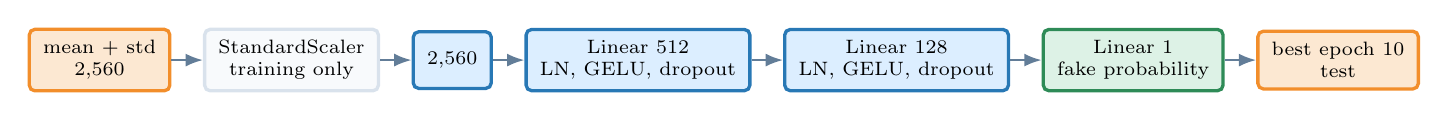
\begin{tikzpicture}[node distance=4mm]
    \node[procorange] (a) {mean + std\\2,560};
    \node[proc,right=of a] (b) {StandardScaler\\training only};
    \node[procblue,right=of b] (c) {2,560};
    \node[procblue,right=of c] (d) {Linear 512\\LN, GELU, dropout};
    \node[procblue,right=of d] (e) {Linear 128\\LN, GELU, dropout};
    \node[procgreen,right=of e] (f) {Linear 1\\fake probability};
    \node[procorange,right=of f] (g) {best epoch 10\\test};
    \draw[flow] (a)--(b); \draw[flow] (b)--(c); \draw[flow] (c)--(d); \draw[flow] (d)--(e);
    \draw[flow] (e)--(f); \draw[flow] (f)--(g);
  \end{tikzpicture}}
  \vspace{0.42cm}
  \begin{columns}[T,onlytextwidth]
    \column{0.42\textwidth}
      \begin{itemize}
        \item AdamW and binary cross-entropy with logits.
        \item Batch size 128, dropout 0.30.
        \item Early stopping uses validation balanced accuracy.
      \end{itemize}
      \vspace{0.15cm}
      \keymetric{Blue}{0.9696}{test balanced accuracy}
    \column{0.56\textwidth}
      \centering
      \begin{tikzpicture}
        \begin{axis}[width=\linewidth,height=4.15cm,xlabel={Epoch},ylabel={Binary cross-entropy},
          tick label style={font=\tiny},label style={font=\scriptsize},legend style={font=\tiny,draw=none,fill=none},
          grid=major,grid style={Rule},axis line style={Rule},legend pos=north east]
          \addplot[Blue,thick] table[x=step,y=train_loss,col sep=comma]{../results/mlp/seed42_20260916T144953Z_mean_std/history.csv};
          \addplot[Orange,thick] table[x=step,y=val_loss,col sep=comma]{../results/mlp/seed42_20260916T144953Z_mean_std/history.csv};
          \addplot[Muted,dashed,thick] coordinates {(10,0) (10,0.24)};
          \legend{training,validation,best epoch}
        \end{axis}
      \end{tikzpicture}
  \end{columns}
\end{frame}

% 10
\begin{frame}{CNN spatial head: end-to-end pipeline}
  \centering
  \resizebox{0.97\textwidth}{!}{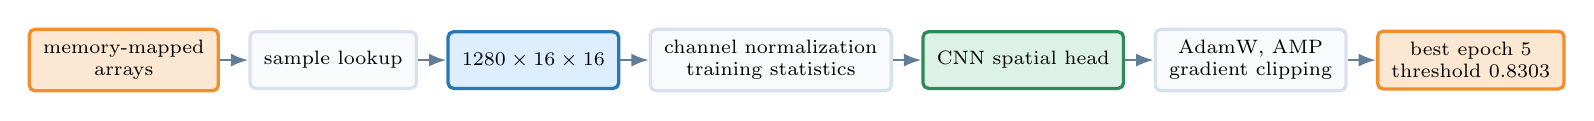
\begin{tikzpicture}[node distance=3.6mm]
    \node[procorange] (a) {memory-mapped\\arrays};
    \node[proc,right=of a] (b) {sample lookup};
    \node[procblue,right=of b] (c) {\(1280\times16\times16\)};
    \node[proc,right=of c] (d) {channel normalization\\training statistics};
    \node[procgreen,right=of d] (e) {CNN spatial head};
    \node[proc,right=of e] (f) {AdamW, AMP\\gradient clipping};
    \node[procorange,right=of f] (g) {best epoch 5\\threshold 0.8303};
    \draw[flow] (a)--(b); \draw[flow] (b)--(c); \draw[flow] (c)--(d); \draw[flow] (d)--(e);
    \draw[flow] (e)--(f); \draw[flow] (f)--(g);
  \end{tikzpicture}}
  \vspace{0.42cm}
  \begin{columns}[T,onlytextwidth]
    \column{0.42\textwidth}
      \begin{columns}[T,onlytextwidth]
        \column{0.53\textwidth}\centering{\color{Blue}\bfseries\fontsize{17}{19}\selectfont 238,993}\par{\color{Muted}\scriptsize trainable parameters}
        \column{0.47\textwidth}\centering{\color{Green}\bfseries\fontsize{19}{21}\selectfont 0.9691}\par{\color{Muted}\scriptsize test balanced accuracy}
      \end{columns}
      \vspace{0.45cm}
      \begin{itemize}
        \item Batch size 8 on CUDA.
        \item 277.7 s recorded training time.
        \item 0.95 MiB TorchScript artifact.
      \end{itemize}
    \column{0.56\textwidth}
      \centering
      \begin{tikzpicture}
        \begin{axis}[width=\linewidth,height=4.1cm,xlabel={Epoch},ylabel={Binary cross-entropy},
          tick label style={font=\tiny},label style={font=\scriptsize},legend style={font=\tiny,draw=none,fill=none},
          grid=major,grid style={Rule},axis line style={Rule},legend pos=north east]
          \addplot[Blue,thick] table[x=step,y=train_loss,col sep=comma]{../results/cnn_spatial_head/seed42_20260917T082650Z/history.csv};
          \addplot[Orange,thick] table[x=step,y=val_loss,col sep=comma]{../results/cnn_spatial_head/seed42_20260917T082650Z/history.csv};
          \addplot[Muted,dashed,thick] coordinates {(5,0) (5,0.42)};
          \legend{training,validation,best epoch}
        \end{axis}
      \end{tikzpicture}
  \end{columns}
\end{frame}

% 11
\begin{frame}{CNN spatial head architecture}
  \centering
  \resizebox{0.97\textwidth}{!}{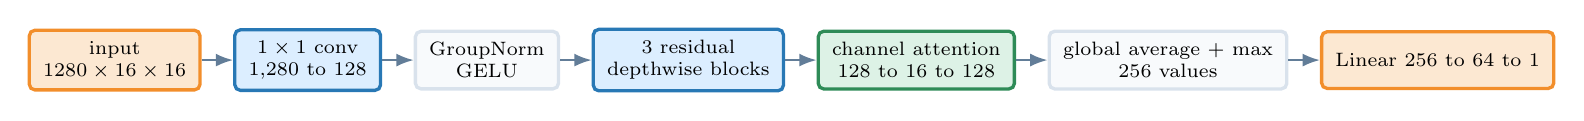
\begin{tikzpicture}[node distance=4mm]
    \node[procorange] (a) {input\\\(1280\times16\times16\)};
    \node[procblue,right=of a] (b) {\(1\times1\) conv\\1,280 to 128};
    \node[proc,right=of b] (c) {GroupNorm\\GELU};
    \node[procblue,right=of c] (d) {3 residual\\depthwise blocks};
    \node[procgreen,right=of d] (e) {channel attention\\128 to 16 to 128};
    \node[proc,right=of e] (f) {global average + max\\256 values};
    \node[procorange,right=of f] (g) {Linear 256 to 64 to 1};
    \draw[flow] (a)--(b); \draw[flow] (b)--(c); \draw[flow] (c)--(d); \draw[flow] (d)--(e);
    \draw[flow] (e)--(f); \draw[flow] (f)--(g);
  \end{tikzpicture}}
  \vspace{0.42cm}
  \begin{columns}[T,onlytextwidth]
    \column{0.49\textwidth}
      {\color{Navy}\bfseries Residual depthwise block}\par\vspace{0.2cm}
      \centering
      \resizebox{0.96\linewidth}{!}{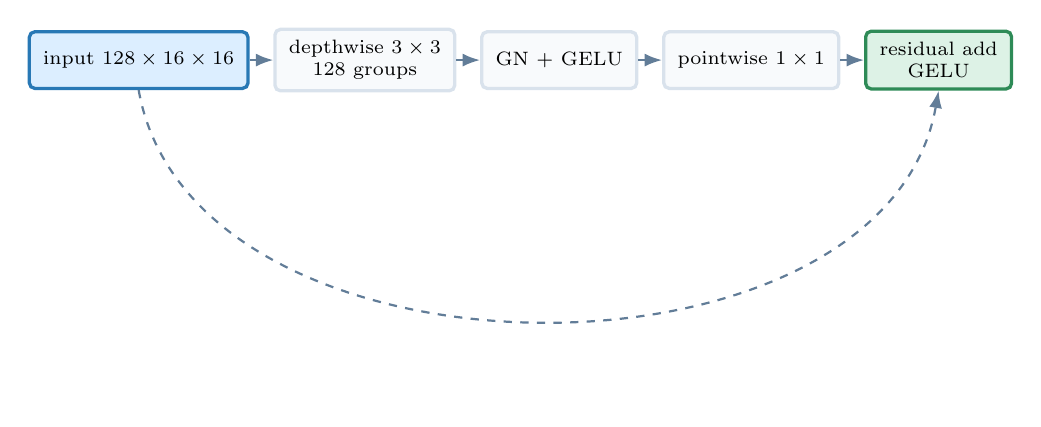
\begin{tikzpicture}[node distance=3mm]
        \node[procblue] (x) {input \(128\times16\times16\)};
        \node[proc,right=of x] (a) {depthwise \(3\times3\)\\128 groups};
        \node[proc,right=of a] (b) {GN + GELU};
        \node[proc,right=of b] (c) {pointwise \(1\times1\)};
        \node[procgreen,right=of c] (d) {residual add\\GELU};
        \draw[flow] (x)--(a); \draw[flow] (a)--(b); \draw[flow] (b)--(c); \draw[flow] (c)--(d);
        \draw[dashflow] (x.south) to[out=-80,in=-100] (d.south);
      \end{tikzpicture}}
    \column{0.49\textwidth}
      {\color{Navy}\bfseries Channel attention}\par\vspace{0.2cm}
      \centering
      \resizebox{0.96\linewidth}{!}{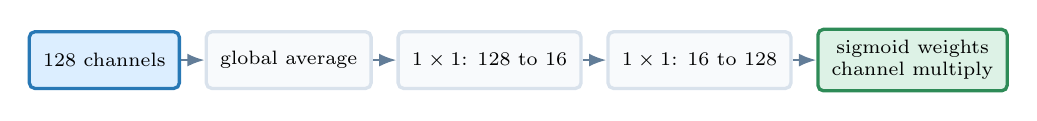
\begin{tikzpicture}[node distance=3mm]
        \node[procblue] (x) {128 channels};
        \node[proc,right=of x] (a) {global average};
        \node[proc,right=of a] (b) {\(1\times1\): 128 to 16};
        \node[proc,right=of b] (c) {\(1\times1\): 16 to 128};
        \node[procgreen,right=of c] (d) {sigmoid weights\\channel multiply};
        \draw[flow] (x)--(a); \draw[flow] (a)--(b); \draw[flow] (b)--(c); \draw[flow] (c)--(d);
      \end{tikzpicture}}
  \end{columns}
  \vfill
  {\scriptsize\color{Muted}Depthwise convolutions preserve local structure efficiently. Attention reweights the most informative latent channels.}
\end{frame}

% 12
\begin{frame}{Compact ConvNeXt: end-to-end pipeline}
  \centering
  \resizebox{0.97\textwidth}{!}{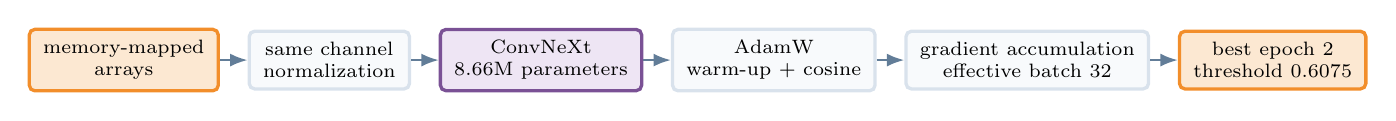
\begin{tikzpicture}[node distance=3.5mm]
    \node[procorange] (a) {memory-mapped\\arrays};
    \node[proc,right=of a] (b) {same channel\\normalization};
    \node[procpurple,right=of b] (c) {ConvNeXt\\8.66M parameters};
    \node[proc,right=of c] (d) {AdamW\\warm-up + cosine};
    \node[proc,right=of d] (e) {gradient accumulation\\effective batch 32};
    \node[procorange,right=of e] (f) {best epoch 2\\threshold 0.6075};
    \draw[flow] (a)--(b); \draw[flow] (b)--(c); \draw[flow] (c)--(d); \draw[flow] (d)--(e); \draw[flow] (e)--(f);
  \end{tikzpicture}}
  \vspace{0.28cm}
  \begin{columns}[T,onlytextwidth]
    \column{0.42\textwidth}
      \keymetric{Purple}{0.9565}{test balanced accuracy}
      \vspace{0.42cm}
      \begin{itemize}
        \item CPU-only PyTorch build in the recorded run.
        \item Physical batch size 2, accumulation 16.
        \item 2,248.3 s training time and 33.18 MiB artifact.
      \end{itemize}
    \column{0.56\textwidth}
      \centering
      \begin{tikzpicture}
        \begin{axis}[width=\linewidth,height=3.85cm,xlabel={Epoch},ylabel={Binary cross-entropy},
          xtick={1,2,3,4},tick label style={font=\tiny},label style={font=\scriptsize},
          legend style={font=\tiny,draw=none,fill=none},grid=major,grid style={Rule},axis line style={Rule},legend pos=north west]
          \addplot[Blue,thick,mark=*] table[x=step,y=train_loss,col sep=comma]{../results/convnext/seed42_20260917T111244Z/history.csv};
          \addplot[Orange,thick,mark=*] table[x=step,y=val_loss,col sep=comma]{../results/convnext/seed42_20260917T111244Z/history.csv};
          \addplot[Muted,dashed,thick] coordinates {(2,0.04) (2,0.21)};
          \legend{training,validation,best epoch}
        \end{axis}
      \end{tikzpicture}
  \end{columns}
\end{frame}

% 13
\begin{frame}{\strut Compact ConvNeXt architecture}
  \centering
  \resizebox{0.94\textwidth}{!}{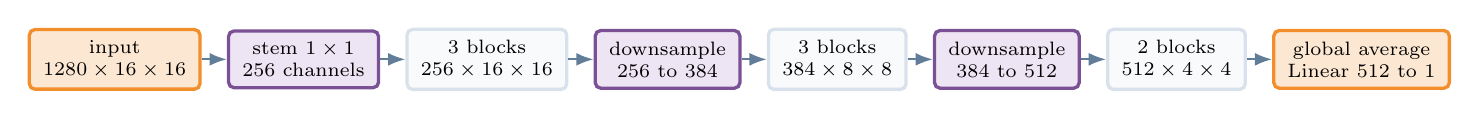
\begin{tikzpicture}[node distance=3.2mm]
    \node[procorange] (a) {input\\\(1280\times16\times16\)};
    \node[procpurple,right=of a] (b) {stem \(1\times1\)\\256 channels};
    \node[proc,right=of b] (c) {3 blocks\\\(256\times16\times16\)};
    \node[procpurple,right=of c] (d) {downsample\\256 to 384};
    \node[proc,right=of d] (e) {3 blocks\\\(384\times8\times8\)};
    \node[procpurple,right=of e] (f) {downsample\\384 to 512};
    \node[proc,right=of f] (g) {2 blocks\\\(512\times4\times4\)};
    \node[procorange,right=of g] (h) {global average\\Linear 512 to 1};
    \draw[flow] (a)--(b); \draw[flow] (b)--(c); \draw[flow] (c)--(d); \draw[flow] (d)--(e);
    \draw[flow] (e)--(f); \draw[flow] (f)--(g); \draw[flow] (g)--(h);
  \end{tikzpicture}}
  \vspace{0.38cm}
  \begin{columns}[T,onlytextwidth]
    \column{0.58\textwidth}
      {\color{Navy}\bfseries One ConvNeXt block}\par\vspace{0.2cm}
      \centering
      \resizebox{0.94\linewidth}{!}{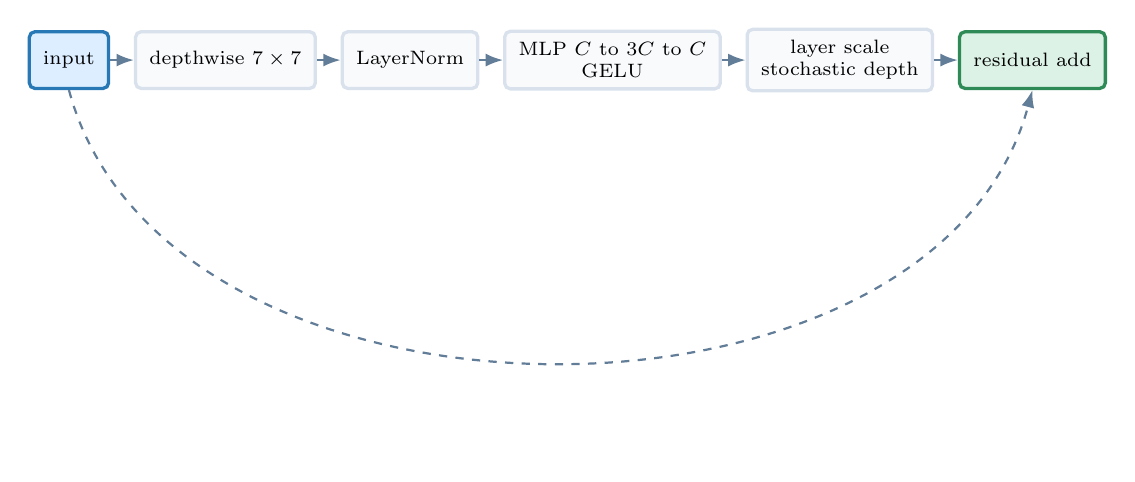
\begin{tikzpicture}[node distance=3mm]
        \node[procblue] (x) {input};
        \node[proc,right=of x] (a) {depthwise \(7\times7\)};
        \node[proc,right=of a] (b) {LayerNorm};
        \node[proc,right=of b] (c) {MLP \(C\) to \(3C\) to \(C\)\\GELU};
        \node[proc,right=of c] (d) {layer scale\\stochastic depth};
        \node[procgreen,right=of d] (e) {residual add};
        \draw[flow] (x)--(a); \draw[flow] (a)--(b); \draw[flow] (b)--(c); \draw[flow] (c)--(d); \draw[flow] (d)--(e);
        \draw[dashflow] (x.south) to[out=-75,in=-105] (e.south);
      \end{tikzpicture}}
    \column{0.39\textwidth}
      \small
      \begin{tabular}{@{}rrrr@{}}
        \toprule
        Stage & \(C\) & \(3C\) & Blocks\\
        \midrule
        1 & 256 & 768 & 3\\
        2 & 384 & 1,152 & 3\\
        3 & 512 & 1,536 & 2\\
        \bottomrule
      \end{tabular}
      \vspace{0.35cm}
      {\scriptsize\color{Muted}Spatial resolution decreases from 16 to 8 to 4 while channel capacity increases.}
  \end{columns}
\end{frame}

% 14
\begin{frame}{Calibrated ensemble pipeline}
  \centering
  \resizebox{0.96\textwidth}{!}{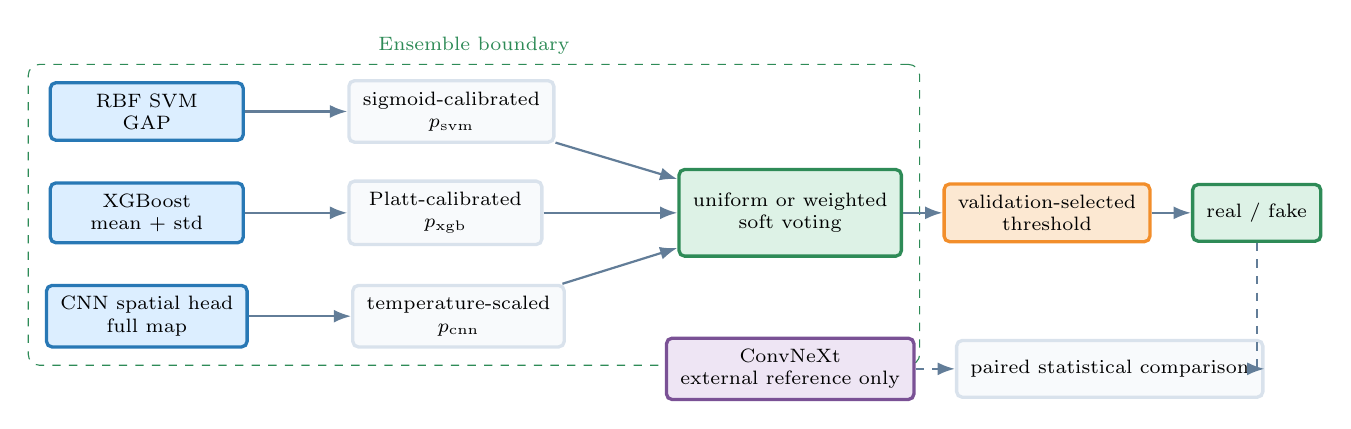
\begin{tikzpicture}[node distance=5mm]
    \node[procblue,minimum width=2.45cm] (s) {RBF SVM\\GAP};
    \node[procblue,below=of s,minimum width=2.45cm] (x) {XGBoost\\mean + std};
    \node[procblue,below=of x,minimum width=2.45cm] (c) {CNN spatial head\\full map};
    \node[proc,right=13mm of s,minimum width=2.45cm] (sp) {sigmoid-calibrated\\\(p_{\mathrm{svm}}\)};
    \node[proc,right=13mm of x,minimum width=2.45cm] (xp) {Platt-calibrated\\\(p_{\mathrm{xgb}}\)};
    \node[proc,right=13mm of c,minimum width=2.45cm] (cp) {temperature-scaled\\\(p_{\mathrm{cnn}}\)};
    \node[procgreen,right=17mm of xp,minimum width=2.5cm,minimum height=1.1cm] (v) {uniform or weighted\\soft voting};
    \node[procorange,right=of v,minimum width=2.25cm] (t) {validation-selected\\threshold};
    \node[procgreen,right=of t] (y) {real / fake};
    \draw[flow] (s)--(sp); \draw[flow] (x)--(xp); \draw[flow] (c)--(cp);
    \draw[flow] (sp)--(v); \draw[flow] (xp)--(v); \draw[flow] (cp)--(v); \draw[flow] (v)--(t); \draw[flow] (t)--(y);
    \node[procpurple,below=10mm of v] (cn) {ConvNeXt\\external reference only};
    \node[proc,right=of cn] (cmp) {paired statistical comparison};
    \draw[dashflow] (cn)--(cmp); \draw[dashflow] (y.south) |- (cmp.east);
    \begin{scope}[on background layer]
      \node[draw=Green,dashed,rounded corners=4pt,fit=(s)(c)(v),inner sep=6pt,label={[font=\scriptsize,text=Green]above:Ensemble boundary}] {};
    \end{scope}
  \end{tikzpicture}}
  \vfill
  \begin{columns}[T,onlytextwidth]
    \column{0.32\textwidth}\centering\textbf{SVM}\par{\scriptsize global nonlinear boundary}
    \column{0.32\textwidth}\centering\textbf{XGBoost}\par{\scriptsize threshold interactions}
    \column{0.32\textwidth}\centering\textbf{CNN}\par{\scriptsize local spatial evidence}
  \end{columns}
\end{frame}

% 15
\begin{frame}{How weighted soft voting works}
  \begin{columns}[T,onlytextwidth]
    \column{0.56\textwidth}
      \centering
      \resizebox{\linewidth}{!}{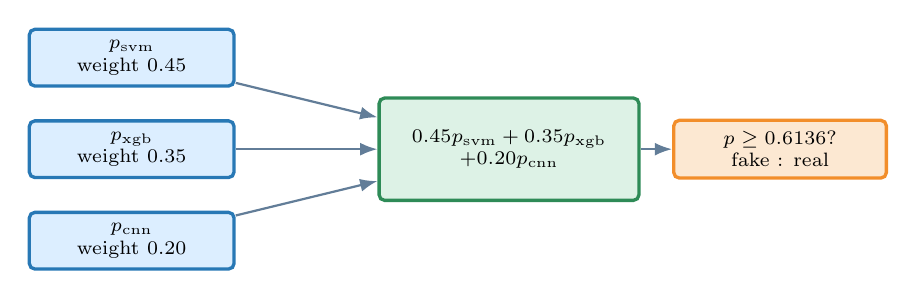
\begin{tikzpicture}[node distance=4mm]
        \node[procblue,minimum width=2.6cm] (s) {\(p_{\mathrm{svm}}\)\\weight 0.45};
        \node[procblue,below=of s,minimum width=2.6cm] (x) {\(p_{\mathrm{xgb}}\)\\weight 0.35};
        \node[procblue,below=of x,minimum width=2.6cm] (c) {\(p_{\mathrm{cnn}}\)\\weight 0.20};
        \node[procgreen,right=18mm of x,minimum width=3.3cm,minimum height=1.3cm] (sum) {\(0.45p_{\mathrm{svm}}+0.35p_{\mathrm{xgb}}\)\\\(+0.20p_{\mathrm{cnn}}\)};
        \node[procorange,right=of sum,minimum width=2.7cm] (thr) {\(p\geq0.6136\)?\\fake : real};
        \draw[flow] (s)--(sum); \draw[flow] (x)--(sum); \draw[flow] (c)--(sum); \draw[flow] (sum)--(thr);
      \end{tikzpicture}}
      \vspace{0.45cm}
      {\small Uniform voting uses \(p=(p_{\mathrm{svm}}+p_{\mathrm{xgb}}+p_{\mathrm{cnn}})/3\).}
    \column{0.41\textwidth}
      {\color{Navy}\bfseries Illustrative sample}\par\vspace{0.2cm}
      \begin{align*}
        p_{\mathrm{svm}} &= 0.80\\
        p_{\mathrm{xgb}} &= 0.60\\
        p_{\mathrm{cnn}} &= 0.90\\[1mm]
        p_{\mathrm{weighted}} &= 0.75
      \end{align*}
      \vspace{-0.2cm}
      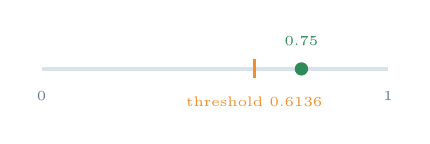
\begin{tikzpicture}
        \draw[very thick,Rule] (0,0)--(4.4,0);
        \draw[very thick,Orange] (2.7,-.12)--(2.7,.12);
        \fill[Green] (3.3,0) circle (2.4pt);
        \node[font=\tiny,text=Muted] at (0,-.35) {0};
        \node[font=\tiny,text=Orange] at (2.7,-.42) {threshold 0.6136};
        \node[font=\tiny,text=Green] at (3.3,.35) {0.75};
        \node[font=\tiny,text=Muted] at (4.4,-.35) {1};
      \end{tikzpicture}
      \vspace{0.25cm}
      {\color{Green}\bfseries Prediction: fake}
  \end{columns}
  \vfill
  {\scriptsize\color{Muted}Weights and threshold were optimized on validation balanced accuracy, then frozen before test evaluation.}
\end{frame}

% 16
\begin{frame}{All models achieve strong test performance}
  \begin{columns}[T,onlytextwidth]
    \column{0.62\textwidth}
      \scriptsize
      \setlength{\tabcolsep}{4.2pt}
      \begin{tabular}{@{}lrrrr@{}}
        \toprule
        \textbf{Model} & \textbf{Bal. acc.} & \textbf{ROC-AUC} & \textbf{PR-AUC} & \textbf{F1 fake}\\
        \midrule
        RBF SVM & \textbf{0.9722} & 0.9971 & 0.9979 & 0.9728\\
        XGBoost & 0.9597 & 0.9934 & 0.9953 & 0.9663\\
        MLP & 0.9696 & 0.9959 & 0.9972 & 0.9715\\
        CNN spatial head & 0.9691 & 0.9970 & 0.9978 & \textbf{0.9732}\\
        Uniform ensemble & 0.9674 & \textbf{0.9974} & 0.9981 & 0.9685\\
        Weighted ensemble & 0.9702 & 0.9974 & \textbf{0.9981} & 0.9714\\
        ConvNeXt & 0.9565 & 0.9933 & 0.9947 & 0.9600\\
        \bottomrule
      \end{tabular}
      \vspace{0.45cm}
      \begin{itemize}
        \item RBF SVM has the highest balanced accuracy.
        \item The ensemble leads on ranking metrics, not thresholded accuracy.
        \item Compact models remain competitive with ConvNeXt.
      \end{itemize}
    \column{0.36\textwidth}
      \centering
      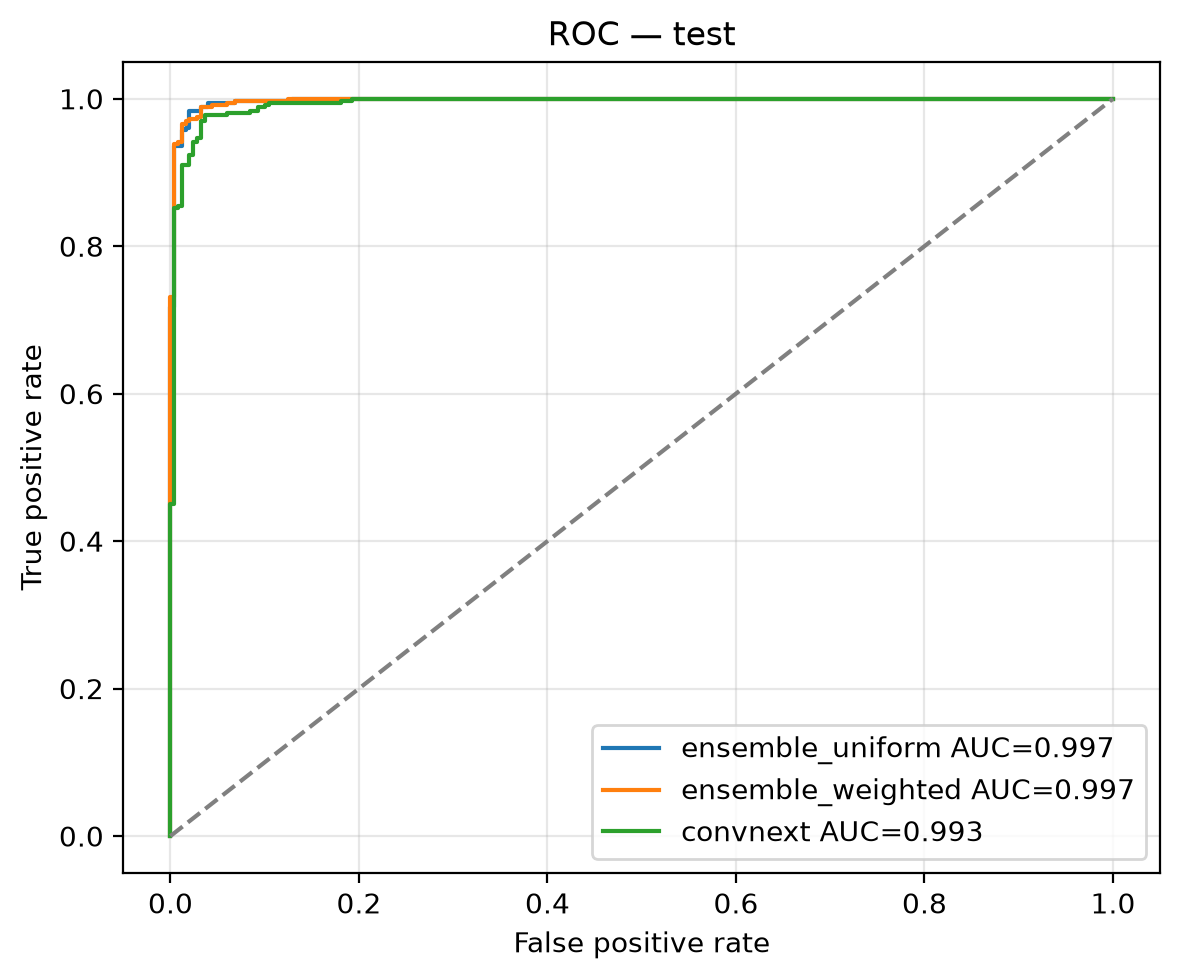
\includegraphics[width=\linewidth]{../results/ensemble/seed42_20260917T122732Z/figures/roc_curve.png}
      \vspace{-0.2cm}
      {\scriptsize\color{Muted}All compared curves exceed 0.99 ROC-AUC.}
  \end{columns}
\end{frame}

% 17
\begin{frame}{Test error profiles}
  \centering
  \begin{columns}[T,onlytextwidth]
    \column{0.32\textwidth}\centering\confmatrix{RBF SVM}{247}{2}{17}{340}
    \column{0.32\textwidth}\centering\confmatrix{Weighted ensemble}{246}{3}{17}{340}
    \column{0.32\textwidth}\centering\confmatrix{ConvNeXt}{242}{7}{21}{336}
  \end{columns}
  \vspace{0.30cm}
  \begin{columns}[T,onlytextwidth]
    \column{0.33\textwidth}\centering{\small\color{Blue}\textbf{19 errors}}\\[-1mm]{\scriptsize 2 false positives, 17 false negatives}
    \column{0.33\textwidth}\centering{\small\color{Green}\textbf{20 errors}}\\[-1mm]{\scriptsize 3 false positives, 17 false negatives}
    \column{0.33\textwidth}\centering{\small\color{Purple}\textbf{28 errors}}\\[-1mm]{\scriptsize 7 false positives, 21 false negatives}
  \end{columns}
  \vspace{0.25cm}
  {\small\color{Navy}\bfseries SVM minimizes false positives. The weighted ensemble reduces ConvNeXt's false negatives from 21 to 17.}
\end{frame}

% 18
\begin{frame}{Why the ensemble still adds value}
  \begin{columns}[T,onlytextwidth]
    \column{0.49\textwidth}
      {\color{Navy}\bfseries Error correlation on test}\par\vspace{0.2cm}
      \centering
      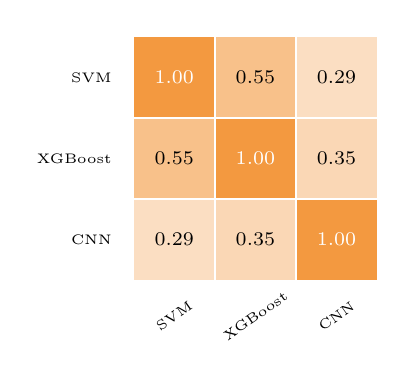
\begin{tikzpicture}[font=\scriptsize]
        \matrix[matrix of nodes,ampersand replacement=\&,nodes={minimum size=1.03cm,anchor=center},
          row sep=0pt,column sep=0pt] (m) {
          |[fill=Orange!90,text=white]|1.00 \& |[fill=Orange!55]|0.55 \& |[fill=Orange!29]|0.29 \\
          |[fill=Orange!55]|0.55 \& |[fill=Orange!90,text=white]|1.00 \& |[fill=Orange!35]|0.35 \\
          |[fill=Orange!29]|0.29 \& |[fill=Orange!35]|0.35 \& |[fill=Orange!90,text=white]|1.00 \\
        };
        \draw[Rule] (m-1-1.north west) rectangle (m-3-3.south east);
        \foreach \i in {1,2,3}{\foreach \j in {1,2,3}{\draw[white] (m-\i-\j.north west) rectangle (m-\i-\j.south east);}}
        \node[rotate=35,font=\tiny] at ($(m-3-1.south)+(0,-.45)$) {SVM};
        \node[rotate=35,font=\tiny] at ($(m-3-2.south)+(0,-.45)$) {XGBoost};
        \node[rotate=35,font=\tiny] at ($(m-3-3.south)+(0,-.45)$) {CNN};
        \node[font=\tiny,anchor=east] at ($(m-1-1.west)+(-.15,0)$) {SVM};
        \node[font=\tiny,anchor=east] at ($(m-2-1.west)+(-.15,0)$) {XGBoost};
        \node[font=\tiny,anchor=east] at ($(m-3-1.west)+(-.15,0)$) {CNN};
      \end{tikzpicture}
      \vspace{0.20cm}
      {\scriptsize\color{Muted}Probability correlation: 0.953--0.971.\\Error correlation: 0.294--0.546.}
    \column{0.49\textwidth}
      {\color{Navy}\bfseries Unique correct cases}\par\vspace{0.2cm}
      \centering
      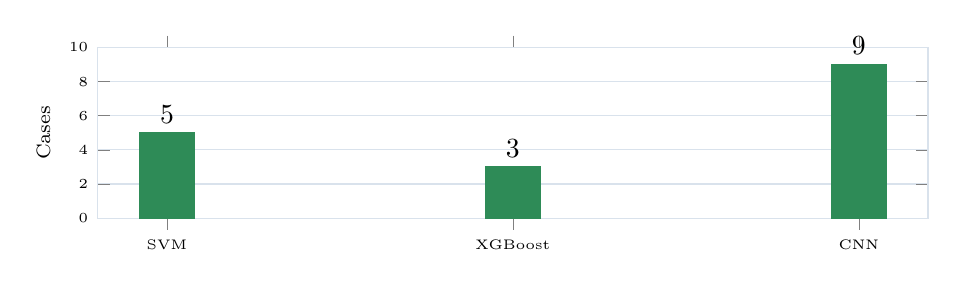
\begin{tikzpicture}
        \begin{axis}[width=\linewidth,height=3.75cm,ybar,bar width=20pt,ymin=0,ymax=10,
          symbolic x coords={SVM,XGBoost,CNN},xtick=data,ylabel={Cases},
          nodes near coords,tick label style={font=\tiny},label style={font=\scriptsize},
          axis line style={Rule},ymajorgrids=true,grid style={Rule}]
          \addplot[fill=Green,draw=Green] coordinates {(SVM,5) (XGBoost,3) (CNN,9)};
        \end{axis}
      \end{tikzpicture}
      \vspace{-0.2cm}
      {\scriptsize\color{Muted}Brier score: uniform 0.0187; weighted 0.0196.}
  \end{columns}
  \vspace{-0.02cm}
  {\small\color{Navy}\bfseries Similar probability rankings coexist with complementary errors.}
\end{frame}

% 19
\begin{frame}{Ensemble and ConvNeXt are comparable in hard classification}
  \begin{columns}[T,onlytextwidth]
    \column{0.57\textwidth}
      \scriptsize
      \begin{tabular}{@{}p{2.15cm}rr@{}}
        \toprule
        \textbf{Metric} & \textbf{Difference} & \textbf{Paired 95\% CI}\\
        \midrule
        Balanced accuracy & +0.0116 & [-0.0042, 0.0271]\\
        ROC-AUC & +0.0041 & [0.0014, 0.0077]\\
        PR-AUC & +0.0034 & [0.0009, 0.0069]\\
        \bottomrule
      \end{tabular}\par
      \vspace{0.28cm}
      {\color{Navy}\bfseries McNemar test}\par
      \small
      \begin{itemize}
        \item Ensemble-only correct: 18 cases.
        \item ConvNeXt-only correct: 10 cases.
        \item Exact \(p=0.1849\).
      \end{itemize}
      {\scriptsize The ranking metrics favor the ensemble; the hard-decision difference is not statistically significant.}
    \column{0.40\textwidth}
      \centering
      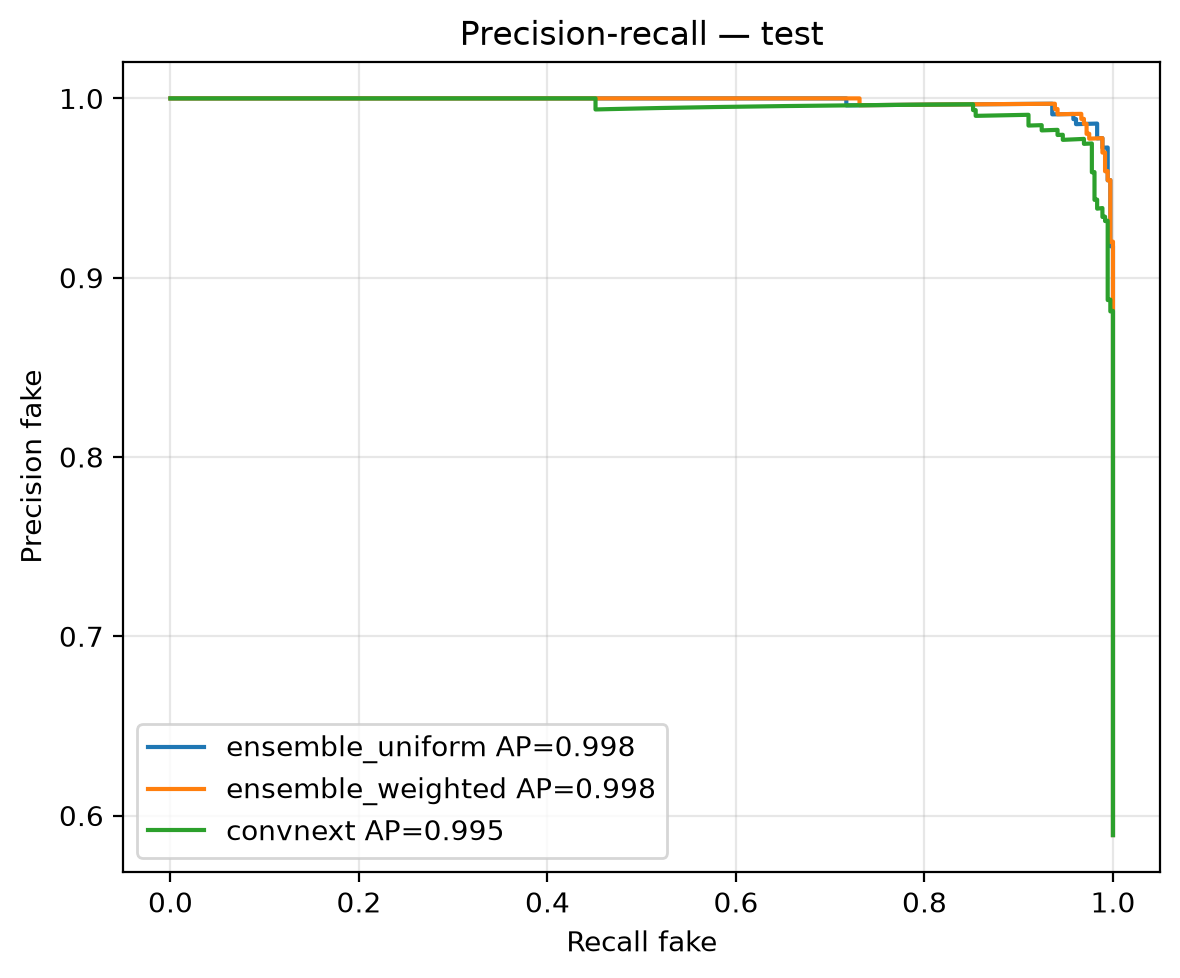
\includegraphics[width=0.90\linewidth]{../results/ensemble/seed42_20260917T122732Z/figures/precision_recall_curve.png}
      \vspace{-0.2cm}
      {\scriptsize\color{Muted}Paired bootstrap favors the ensemble for PR-AUC.}
  \end{columns}
\end{frame}

% 20
\begin{frame}{Conclusions and limitations}
  \begin{columns}[T,onlytextwidth]
    \column{0.48\textwidth}
      {\color{Green}\bfseries Conclusions}\par\vspace{0.25cm}
      \begin{itemize}
        \item Stable Diffusion feature maps provide a strong real/fake signal.
        \item Global channel summaries are sufficient for excellent performance.
        \item RBF SVM leads balanced accuracy at 0.9722.
        \item The ensemble improves ranking and probability quality, with higher point estimates than ConvNeXt.
      \end{itemize}
    \column{0.49\textwidth}
      {\color{Orange}\bfseries Limitations}\par\vspace{0.25cm}
      \begin{itemize}
        \item One random seed and no group-aware split.
        \item Source and preprocessing artifacts may contribute to separability.
        \item Validation supports calibration, thresholds, and ensemble weights.
        \item ConvNeXt used a short CPU-only run.
        \item No unseen-generator or raw-image evaluation.
      \end{itemize}
  \end{columns}
  \vfill
  {\centering\color{Navy}\bfseries Results support practical comparability, not universal model superiority.\par}
\end{frame}

% 21
\begin{frame}{Future work}
  \begin{columns}[T,onlytextwidth]
    \column{0.33\textwidth}
      {\color{Blue}\bfseries Stronger validation}\par\vspace{0.25cm}
      \begin{itemize}
        \item Multiple neural seeds.
        \item Group-aware splits.
        \item Dedicated calibration data.
      \end{itemize}
    \column{0.33\textwidth}
      {\color{Orange}\bfseries Broader generalization}\par\vspace{0.25cm}
      \begin{itemize}
        \item Unseen generators.
        \item Generator attribution.
        \item Cross-source evaluation.
      \end{itemize}
    \column{0.33\textwidth}
      {\color{Green}\bfseries Deployment evidence}\par\vspace{0.25cm}
      \begin{itemize}
        \item Full GPU ConvNeXt schedule.
        \item Raw-image baseline.
        \item Efficiency under one platform.
      \end{itemize}
  \end{columns}
  \vspace{0.55cm}
  \begin{center}
    {\color{Navy}\bfseries\large Internal diffusion representations are promising detection features.}\par
    \vspace{0.25cm}
    {\color{Muted}Robust deployment depends on cross-source and cross-generator generalization.}\par
    \vspace{0.38cm}
    {\color{Blue}\large Questions?}
  \end{center}
\end{frame}

\appendix

% Backup A
\begin{frame}[noframenumbering]{Backup A: Detailed split and class counts}
  \centering
  \begin{tabular}{@{}lrrr@{}}
    \toprule
    \textbf{Split} & \textbf{Total} & \textbf{Real} & \textbf{Fake}\\
    \midrule
    Training & 2,825 & 1,157 & 1,668\\
    Validation & 606 & 248 & 358\\
    Test & 606 & 249 & 357\\
    \bottomrule
  \end{tabular}\par
  \vspace{0.8cm}
  {\small\color{Muted}Shared split hash}\par
  {\ttfamily\scriptsize e23bd01e9ec079e665ed5cb58cdba6c190d40bb702919412e2f5f5aeca63cbd6}
\end{frame}

% Backup B
\begin{frame}[noframenumbering]{Backup B: Efficiency and artifact size}
  \centering
  \small
  \begin{tabular}{@{}lrrr@{}}
    \toprule
    \textbf{Model} & \textbf{Training} & \textbf{Test inference} & \textbf{Artifact}\\
    \midrule
    RBF SVM & 431.8 s & 2.516 s & 55.17 MiB\\
    XGBoost & 1,240.1 s & 0.006 s & 0.25 MiB\\
    MLP & 4.6 s & 0.014 s & 5.27 MiB\\
    CNN spatial head & 277.7 s & 3.209 s & 0.95 MiB\\
    ConvNeXt & 2,248.3 s & 31.099 s & 33.18 MiB\\
    \bottomrule
  \end{tabular}\par
  \vspace{0.65cm}
  {\color{Orange}\bfseries Caution}\par
  Recorded times include different execution paths, tuning budgets, and hardware. They are not a controlled speed benchmark.
\end{frame}

% Backup C
\begin{frame}[noframenumbering]{Backup C: Test confidence intervals}
  \centering
  \small
  \begin{tabular}{@{}lrr@{}}
    \toprule
    \textbf{Model} & \textbf{Balanced accuracy} & \textbf{Bootstrap 95\% CI}\\
    \midrule
    RBF SVM & 0.9722 & [0.9583, 0.9840]\\
    XGBoost & 0.9597 & [0.9434, 0.9754]\\
    CNN spatial head & 0.9691 & [0.9550, 0.9820]\\
    Uniform ensemble & 0.9674 & [0.9534, 0.9801]\\
    Weighted ensemble & 0.9702 & [0.9571, 0.9820]\\
    ConvNeXt & 0.9565 & [0.9407, 0.9718]\\
    \bottomrule
  \end{tabular}
\end{frame}

% Backup D
\begin{frame}[noframenumbering]{Backup D: References}
  \scriptsize
  {\color{Blue}$\bullet$}\quad S. Bonechi, P. Andreini, and B. Toniella Corradini. \emph{Comparing Real and Synthetic Image Representations in Stable Diffusion Models}.\par\medskip
  {\color{Blue}$\bullet$}\quad R. Rombach et al. \emph{High-Resolution Image Synthesis with Latent Diffusion Models}. CVPR, 2022.\par\medskip
  {\color{Blue}$\bullet$}\quad G. Cazenavette et al. \emph{FakeInversion: Learning to Detect Images from Unseen Text-to-Image Models by Inverting Stable Diffusion}. CVPR, 2024.\par\medskip
  {\color{Blue}$\bullet$}\quad T. Chen and C. Guestrin. \emph{XGBoost: A Scalable Tree Boosting System}. KDD, 2016.\par\medskip
  {\color{Blue}$\bullet$}\quad Z. Liu et al. \emph{A ConvNet for the 2020s}. CVPR, 2022.
\end{frame}

% Backup E
\begin{frame}[noframenumbering]{Backup E: Additional diagnostics}
  \begin{columns}[T,onlytextwidth]
    \column{0.49\textwidth}
      \centering
      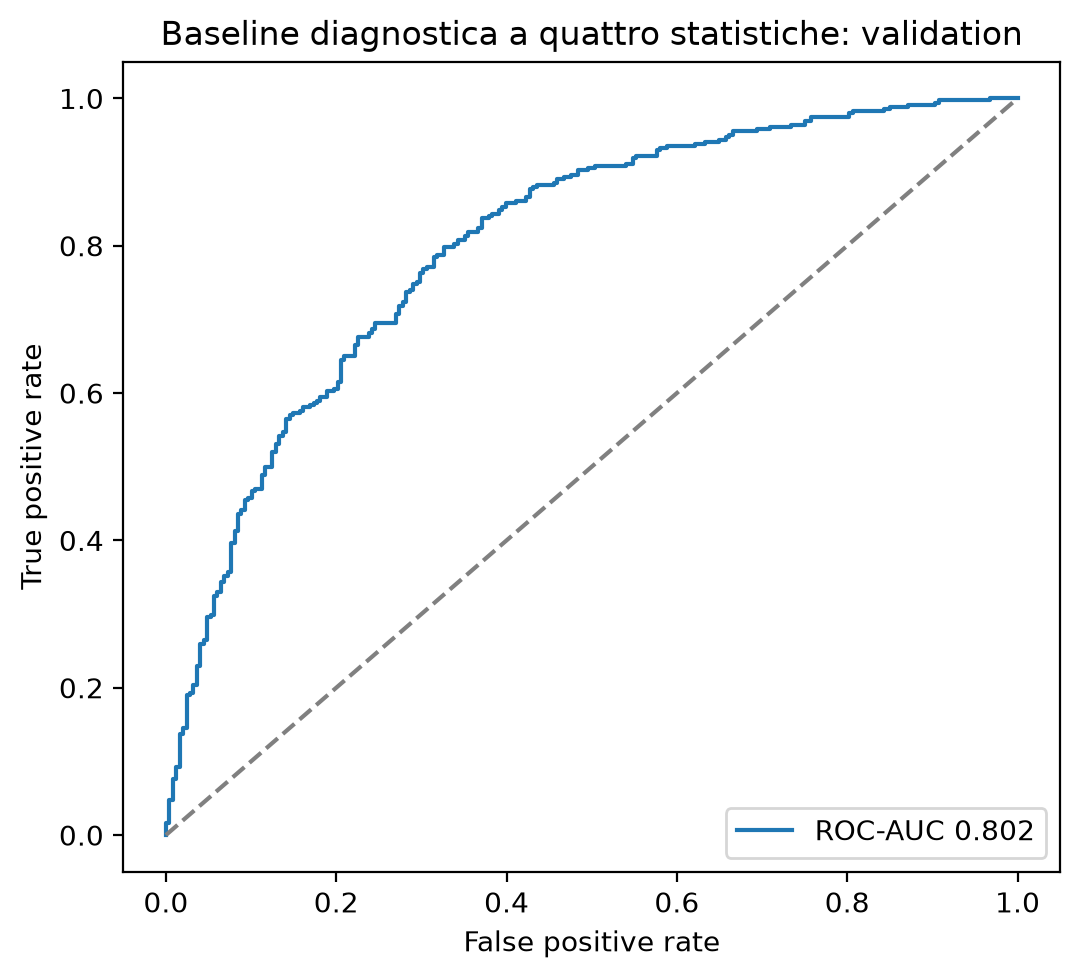
\includegraphics[width=0.83\linewidth,trim=0 0 0 22,clip]{../results/dataset_exploration/seed42_20260916T132745Z/figures/diagnostic_baseline_roc.png}
      \vspace{-0.15cm}
      {\scriptsize\color{Muted}Four-statistic diagnostic baseline.}
    \column{0.49\textwidth}
      \centering
      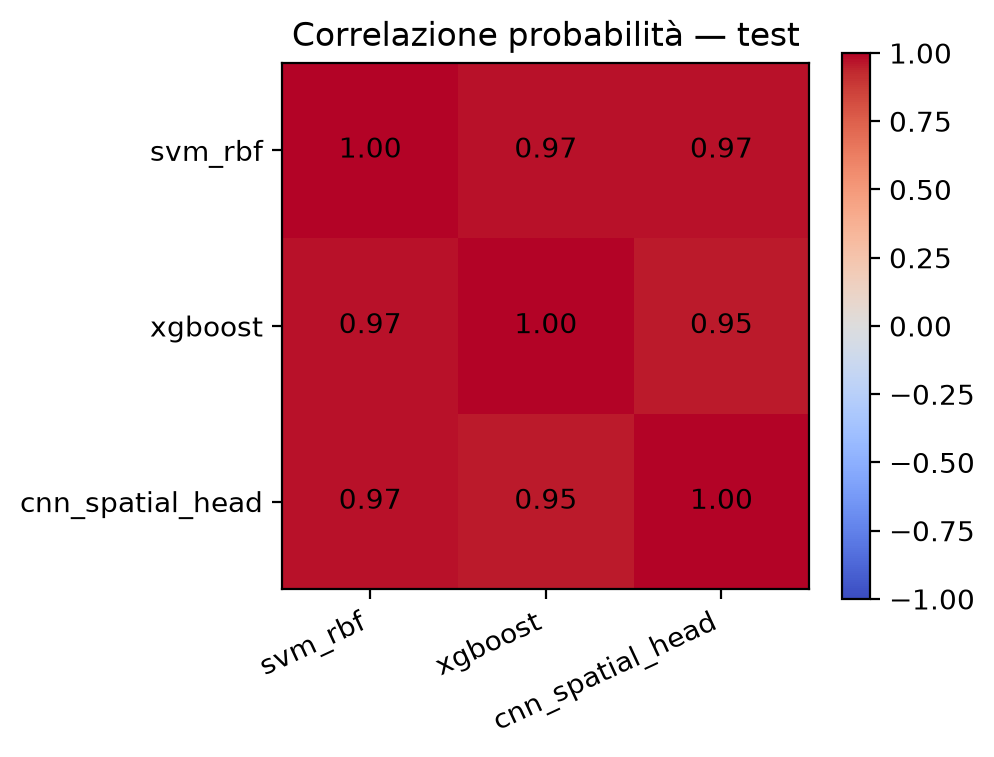
\includegraphics[width=0.83\linewidth,trim=0 0 0 34,clip]{../results/ensemble/seed42_20260917T122732Z/figures/probability_correlation.png}
      \vspace{-0.15cm}
      {\scriptsize\color{Muted}Probability correlation on test.}
  \end{columns}
  \vfill
  {\scriptsize\color{Muted}Further exported diagnostics include top channels, global statistics, probability correlation, near duplicates, and outlier candidates.}
\end{frame}

\end{document}
